\chapter{Сравнение пулковских собственных движений с данными Gaia DR2} \label{ch:ch6}
Первый релиз миссии Gaia содержал собственные движения только для звезд, которые входят в состав каталогов HIPPARCOS и Tycho--2. Это, в основном, звезды до $12^m$ (TGAS). Поэтому в контексте нашего исследования эти данные не давали возможности для полноценного сравнения. Второй релиз миссии Gaia, опубликованный 25 апреля 2018 года, предоставил надежное пятипараметрическое решение (положения, собственные движения и тригонометрические параллаксы) для более чем 1.5 миллиарда звезд  вплоть до $20^m$. Для нас наиболее интересны собственные движения звезд. Как говорилось в главе 3, в рамках изучения быстрых карликов для исследуемых звезд нами  были вычислены и сопоставлены друг с другом собственные движения, полученные на различных по длительности временных базах. Среди исследованных звезд 121 звезда показала значимые различия в величинах собственных движений, что позволило нам отнести их к кандидатам в $\Delta\mu$--двойные. Логичным решением стало использование данных Gaia для проверки наших результатов.

В результате сравнения выяснено, что примерно половина звезд с собственными движениями более 300 mas/yr отсутствует в Gaia DR2. Это не является неожиданностью. Специалисты команды Gaia упоминают в своих работах \cite{2018A&A...616A...2L} упоминают о трудностях кросс--идентификации от скана к скану для звезд с большими собственными движениями.

В общей сложности из всей пулковской программы в Gaia DR2 представлено 684 звезды. Средние значения разностей собственных движений вида (Пулково -- Gaia DR2) весьма малы: $-0.3\pm5.8$~mas/yr по прямому восхождению и $0.3\pm5.6$~mas/yr по склонению. Это подтверждает заявленную среднюю точность пулковских собственных движений.

Разумеется логично было использовать пулковские собственные движения, полученные по всем доступным данным (временная база порядка 65 лет) как квазисредние, а собственные движения этих звезд из Gaia DR2 как квазимгновенные (временная база 22 месяца!). Всего 62 звезды, которые квалифицированы нами ранее как $\Delta\mu$--двойные присутствуют в Gaia DR2. Из них 30 звезд имеют разности собственных движений  (Пулково -- Gaia DR2) отвечающие критерию $F>2.49$. Рисунок~\ref{fig:FvsD} позволяет проанализировать поведение величин F в зависимости от расстояний до звезд. Наибольшие значения F имеют место для сравнительно близких звезд, что естественно, так как в этом случае видимый размер орбиты фотоцентра больше и эффект легче обнаружить. Для объектов дальше 50 пк значения $F>2.49$ почти не встречаются. Горизонтальные линии отвечают значению $F=2.49$ (величина критерия при богатой астрометрической истории и \glqq гауссовости\grqq\ распределения ошибок) и $F=5.3$ (это случай, когда квазисреднее собственное движение вычислено по 6-ти отдельным положениям).

\begin{figure}[pt]
 \centering
 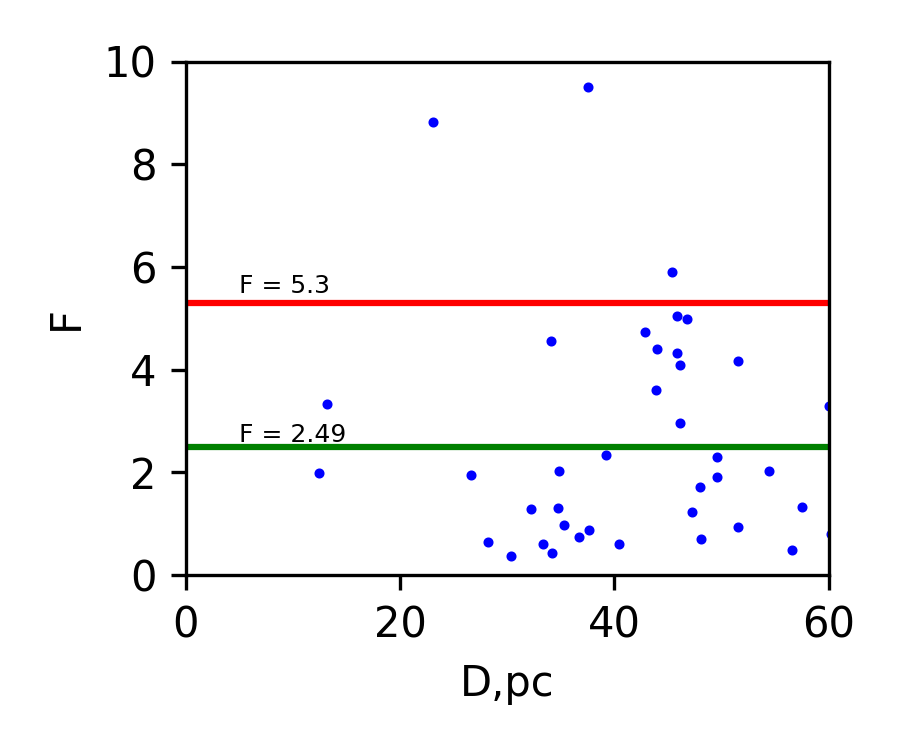
\includegraphics [scale=2] {FvsD}
 \caption{Поведение значения F в зависимости от расстояния до звезд. Звезды с $F>10$ не показаны на графике для удобства его анализа. Часть звезд имеет параллаксы, отвечающими расстояниям более 60 пк. Они были включены в программу наблюдений задолго до появления релизов Gaia, когда величина собственного движения была единственным критерием выбора близких звезд. Процент таких звезд довольно большой "--- около 10\,\%.}
 \label{fig:FvsD}
\end{figure}

Тот факт, что только половина ранее выявленных $\Delta\mu$--двойных подтверждается сравнением с Gaia DR2 демонстрирует недостаток нашего исследования: квази-мгновенные собственные движения вычислялись на основе очень малого числа точек (от 2 до 6). Это могло приводить к тому, что большие значения F были результатом просто больших случайных ошибок квазимгновенных собственных движений. Тем не менее, сравнение с Gaia DR2 показывает значительный процент звезд кандидатов в $\Delta\mu$--двойные, которые сохранили свой статус при использовании более точных данных. В таблице \ref{tab:pul-gaia} приведены данные для 10 звезд с наибольшим значением получившегося параметра F.

\begin{table} [htbp]
	\centering
	\caption{Сравнение собственных движений близких карликов, рассчитанных в Пулкове, с данными Gaia DR2.}%
	\label{tab:pul-gaia}%
	\begin{tabularx}{\textwidth}{ c | c | c | c |c | c | c | c }
	  \hline
           & \multicolumn{2}{c|}{Pulkovo-Gaia DR2} &   \multicolumn{2}{c|}{Pulkovo}    &   \multicolumn{2}{c|}{Gaia DR2}    &       \\ \cline{2-7}
 LSPM ID   &    $\Delta\mu_{RA}$    &   $\Delta\mu_{Dec}$   & $\epsilon\mu_{RA}$ & $\epsilon\mu_{Dec}$ & $\epsilon\mu_{RA}$  & $\epsilon\mu_{Dec}$ & F     \\ \cline{2-7}
           &        \multicolumn{6}{c|}{mas/yr}            &       \\ \hline
J0608+4902 & -11.415 &   9.326 & 1.3  &  2.1  & 0.370 & 0.369 & 9.511 \\
J1931+6843 &  35.419 &  -6.355 & 4.9  &  1.2  & 0.365 & 0.349 & 8.822 \\
J2214+3214 &  -2.886 &  -2.213 & 0.4  &  1.5  & 0.105 & 0.143 & 7.129 \\
J1555+3148 &  11.079 &   6.120 & 3.6  &  1.0  & 0.069 & 0.082 & 6.832 \\
J0850+3239 &  -6.774 &   8.172 & 0.8  &  5.2  & 0.695 & 0.529 & 6.580 \\
J0002+4343 &  19.020 & -30.280 & 3.3  & 14.6  & 0.055 & 0.034 & 6.125 \\
J0836+3902 & -21.748 & -19.643 & 7.1  &  3.9  & 0.125 & 0.088 & 5.894 \\
J2314+3345 & -32.355 &   5.541 & 5.6  &  7.4  & 0.055 & 0.046 & 5.826 \\
J0259+3318 &  -0.657 & 115.582 & 0.6  & 22.3  & 0.069 & 0.064 & 5.296 \\
J2240+6454 &   6.168 & -10.397 & 1.8  &  2.8  & 0.043 & 0.035 & 5.052 \\
\hline
	\end{tabularx}%
\end{table}

После выхода Gaia DR2 многие исследователи стали использовать подходы к выявлению двойных систем частично основанные на сравнении различных наборов собственных движений с данными Gaia. Мы планируем продолжить исследования в этом направлении. Наше конкурентное преимущество могут обеспечить старые фотопластинки из стеклотеки Пулковской обсерватории, которые дают большие разности эпох для вывода независимых квазисредних собственных движений. Но это исследование выходит за рамки данной работы. Здесь мы защищаем методы поиска двойных систем и уже полученные нами результаты.